\documentclass{beamer}
\usepackage[utf8]{inputenc}
\usepackage[T1]{fontenc}
\usepackage[english]{babel}
\usepackage{lmodern}
\usepackage{amsmath}
\usepackage{amssymb}
\usepackage{amsthm}
\usepackage[superscript]{cite}
\usepackage{nicefrac}
\usepackage{upgreek}
\usepackage{stmaryrd}
\usepackage{tikz}
\usepackage{graphicx}
\usepackage{qtree}
\usepackage{dsfont}
\usepackage{eurosym}
\usepackage{tabulary}
\usepackage{setspace}
% \usepackage[colorlinks=true,linkcolor=blue]{hyperref}				% Blaue Links sehen meiner Ansicht nach besser aus als die rot umrandeten Verweise

\usetheme{Madrid}				% Verwende Goettingen für TOC auf jeder Seite, Madrid ohne Navigation

% Kommandos, Operatoren, etc.
\newcommand{\abs}[1]{\lvert#1\rvert}
\newcommand{\norm}[1]{\lVert#1\rVert}
\DeclareMathOperator{\thetafunc}{\uptheta}

% ENDE PRÄAMBEL

\AtBeginSection[]{
	\begin{frame}
		\vfill
		\centering
		\begin{beamercolorbox}[sep=8pt,center,shadow=true,rounded=true]{title}
			\usebeamerfont{title}\insertsectionhead\par%
		\end{beamercolorbox}
		\vfill
	\end{frame}
}

\author{Dominik Blank}
\title{ROI Testing}
\institute{Georg-August-Universität Göttingen}

\setlength{\parindent}{0pt}
\allowdisplaybreaks

\begin{document}

\begin{frame}
	\maketitle
\end{frame}

\begin{frame}
	\tableofcontents
\end{frame}

\section{ROI Testing}

\subsection{The statistical model}

\begin{frame}
	Let $M, N \in \mathbb{N}$ and $G = \left\{ 0, \dots, M-1 \right\} \times  \left\{ 0, \dots, N-1 \right\}$. Assume we are given data
	\begin{equation*}\label{f}
		f(i, j) = c + v(i, j) + \varepsilon_{i, j}
	\end{equation*}
	\begin{itemize}
		\item $(i, j) \in G$
		\item $c \in \mathbb{R}$ is constant
		\item $v: G \to \{ 0, \pm c \}$
		\item $\varepsilon_{m, n} \sim \mathcal{N}(0, \sigma^2)$ i.i.d. normal distributed random variables
	\end{itemize}
	
	Assumption 1: The image $f$ contains a rectangular region of interest.
	Assumption 2: The ROI has a checkerboard pattern.
\end{frame}

\begin{frame}
	\begin{figure}
		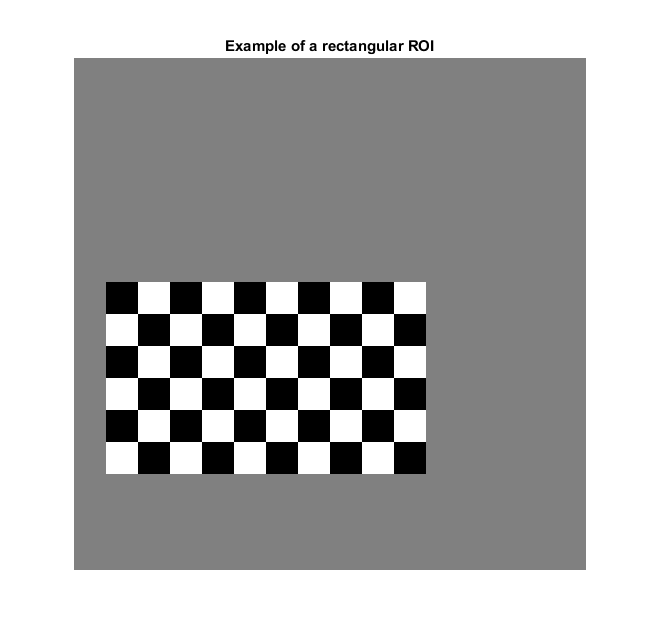
\includegraphics[width=0.6\linewidth]{Testing/ROI}
		\caption[ROI]{Example of a possible region of interest. ($M = 16$, $N = 16$)}
		\label{fig:ROI}
	\end{figure}
\end{frame}

\begin{frame}
	\begin{figure}
		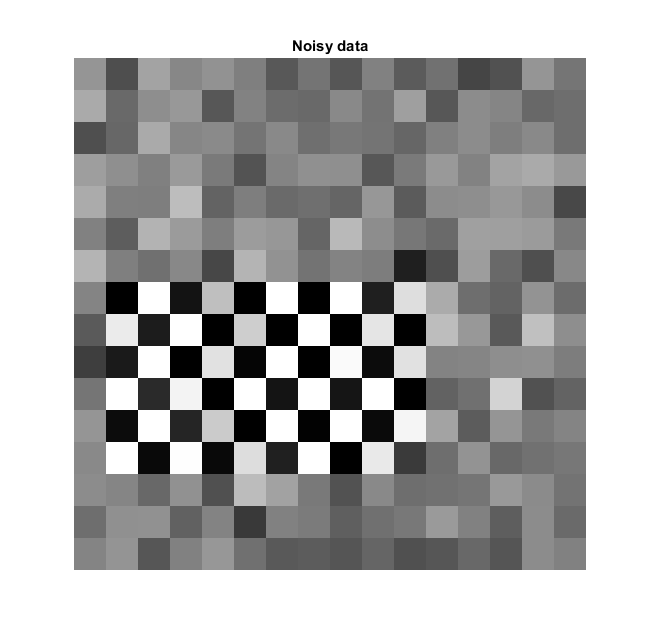
\includegraphics[width=0.6\linewidth]{Testing/ROI_noisy}
		\caption[Noisy ROI]{Same region of interest with noise added. ($\sigma = 30$)}
		\label{fig:ROI_noisy}
	\end{figure}
\end{frame}

\subsection{Testing for the ROI}

\begin{frame}
	\begin{beamercolorbox}[sep=8pt,center,shadow=true,rounded=true]{title}
		Goal: Construct a statistical test for the region of interest.
	\end{beamercolorbox}
\end{frame}

\begin{frame}
	\begin{beamercolorbox}[sep=8pt,center,shadow=true,rounded=true]{title}
		Observation: If a pixel is background, its top and left neighbour pixels or bottom and right neighbour pixels are background as well.
	\end{beamercolorbox}
\end{frame}

\subsubsection{Preparations}

\begin{frame}
	For each pair $(i, j) \in G$ we define four non-observable values
	\begin{align*}
		d_1^\pm(i, j) &= v(i \pm 1, j) - v(i, j) \\
		d_2^\pm(i, j) &= v(i, j \pm 1) - v(i, j)
	\end{align*}
	and combine them to two new values
	\begin{equation*}\label{d}
		d^\pm(i, j) = \sqrt{(v(i \pm 1, j) - v(i, j))^2 + (v(i, j \pm 1) - v(i, j))^2}
	\end{equation*}
\end{frame}

\begin{frame}
	The definition of $d^\pm(i, j)$ helps us define the null hypothesis:
	\begin{equation*}
		H_0 : \min\{ d^+(i, j), d^-(i, j) \} = 0
	\end{equation*}
	Since by definition $d^\pm(i, j) \geq 0$, our alternative hypothesis becomes
	\begin{equation*}
		H_1 : \min\{ d^+(i, j), d^-(i, j) \} > 0
	\end{equation*}
\end{frame}

\begin{frame}
	We also define four observable values
	\begin{align*}
		\tilde{d}^\pm_1(i, j) &= f(i \pm 1, j) - f(i, j) \\
		\tilde{d}^\pm_2(i, j) &= f(i, j \pm 1) - f(i, j)
	\end{align*}
	and combine them to
	\begin{equation*}\label{d_tilde}
		\tilde{d}^\pm(i, j) = \sqrt{\tilde{d}_1^\pm(i, j)^2 + \tilde{d}_2^\pm(i, j)^2}
	\end{equation*}
	
	We use $T = \min \{ \tilde{d}^+(i, j), \tilde{d}^-(i, j) \}$ as our test statistic.
\end{frame}

\subsubsection{Distribution of $\mathbb{P}(\tilde{d}^\pm(i, j) \leq t \mid d^\pm(i, j) = d)$}

\begin{frame}
	Since $v$ only takes values in $\{ 0, -c, c \}$, $d^\pm$ also can only attain values in
	\begin{equation*}
		\mathcal{D} = \{ 0, c, 2 c, \sqrt{2} c, \sqrt{5} c, \sqrt{8} c \}
	\end{equation*}
	
	We want to determine the distribution of $\tilde{d}^\pm(i, j)$ conditioned on $d^\pm(i, j) = d$ for some $d \in \mathcal{D}$.
\end{frame}

\begin{frame}
	We get
	\begin{equation*}
		\mathbb{P}(\tilde{d}^\pm(i, j) \leq t \mid d^\pm(i, j) = d) = \mathbb{P}\left( \sqrt{2} \sigma \sqrt{\left( \frac{X_1}{\sqrt{2} \sigma} \right)^2 + \left( \frac{X_2}{\sqrt{2} \sigma} \right)^2} \leq t \right)
	\end{equation*}
	with
	\begin{align*}
		X_1 &= d_1^\pm(i, j) + \varepsilon_{m \pm 1, n} - \varepsilon_{m, n} \sim \mathcal{N}(d_1^\pm(i, j), 2 \sigma^2) \\
		X_2 &= d_2^\pm(i, j) + \varepsilon_{m, n \pm 1} - \varepsilon_{m, n} \sim \mathcal{N}(d_2^\pm(i, j), 2 \sigma^2)
	\end{align*}
\end{frame}

\begin{frame}
	Using the cumulative distribution function of the non-central chi distribution, we obtain
	\begin{align*}
		\mathbb{P}(\tilde{d}^\pm(i, j) \leq t \mid d^\pm(i, j) = d) &= \mathbb{P}\left( \sqrt{\left( \frac{X_1}{\sqrt{2} \sigma} \right)^2 + \left( \frac{X_2}{\sqrt{2} \sigma} \right)^2} \leq \frac{t}{\sqrt{2} \sigma} \right) \\
		&= 1 - Q_1 \left( \frac{d}{\sqrt{2} \sigma}, \frac{t}{\sqrt{2} \sigma} \right)
	\end{align*}
	
	For $d = 0$ this simplifies a lot and we get
	\begin{equation*}
		\mathbb{P}(\tilde{d}^\pm(i, j) \leq t \mid d^\pm(i, j) = 0) = 1 - \exp \left( - \frac{t^2}{4 \sigma^2} \right)
	\end{equation*}
\end{frame}

\subsubsection{Statistical significance}

\begin{frame}
	Using this, we get an upper bound for the probability of a type I error:
	\begin{equation*}
		\mathbb{P}(T \geq t \mid H_0) \leq \exp \left( - \frac{t^2}{4 \sigma^2} \right)
	\end{equation*}
	
	By taking $t = 2 \sigma \sqrt{- \log(\alpha)}$ we thus can assure a statistical significance of $\alpha$.
\end{frame}

\subsubsection{Power of the test}

\begin{frame}
	We are also interested in bounds for the probability of a type II error.
	
	Using results and notations from the previous sections, we get the lower bound
	\begin{equation*}
		\beta = \mathbb{P}(T \leq t \mid H_1) \geq 1 - Q_1 \left( \frac{2 c}{\sigma}, \frac{t}{\sqrt{2} \sigma} \right)
	\end{equation*}
	
	On the other hand, we get the upper bound
	\begin{equation*}
		\beta = \mathbb{P}(T \leq t \mid H_1) \leq 2 \cdot \left( 1 - Q_1 \left( \frac{c}{\sqrt{2} \sigma}, \frac{t}{\sqrt{2} \sigma} \right) \right)
	\end{equation*}
	
	Thus we can conclude, that
	\begin{equation*}
		\beta \in \left[ 1 - Q_1 \left( \frac{2 c}{\sigma}, \frac{t}{\sqrt{2} \sigma} \right), \min \left\{ 2 \cdot \left( 1 - Q_1 \left( \frac{c}{\sqrt{2} \sigma}, \frac{t}{\sqrt{2} \sigma} \right) \right), 1 \right\} \right]
	\end{equation*}
\end{frame}

\subsubsection{Numerical results}

\begin{frame}
	In the case of a grayscale image, we assume $c = 127.5$. For $t = 2 \sigma \sqrt{- \log(\alpha)}$ and $\alpha = 0.05$ we get the following bounds dependent on the standard deviation $\sigma$.
	
	\begin{figure}[h]
		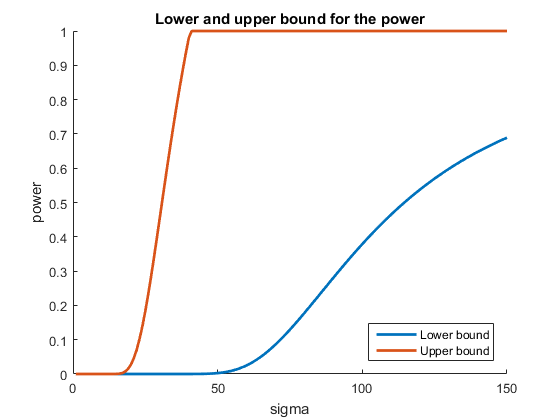
\includegraphics[width=0.6\linewidth]{Testing/Power_Bounds}
		\caption[Power bounds]{For $\alpha = 0.05$ this graph shows the lower and upper bounds for the power of the test for $\sigma \in \{ 1, 2, \dots, 150 \}$.}
		\label{fig:powerbounds}
	\end{figure}
\end{frame}

\begin{frame}
	\begin{itemize}
		\item No type II errors for $\sigma \in \{ 1, 2, \dots, 8 \}$.
		\item Until $\sigma = 21$ the probability of a type II error stays below $\alpha = 0.05$.
		\item Starting at $\sigma = 41$ we can only use the trivial upper bound, i.e. $1$.
		\item The lower bound stays at $0$ until $\sigma = 23$.
		\item At $\sigma = 115$ the lower bound becomes bigger than $0.5$.
	\end{itemize}
\end{frame}

\section{Morphological operations}

\subsection{Opening and closing}

\begin{frame}
	We start by defining erosion and dilation of binary images.
	
	\begin{definition}
		Let $A, B \subseteq \mathbb{R}^m$. The binary erosion of $A$ by $B$ is defined as
		\begin{equation*}
			A \ominus_b B = \left\{ x \in \mathbb{R}^m \mid x + b \in A \; \mathrm{for \; every} \; b \in B \right\}
		\end{equation*}
	\end{definition}
	\begin{definition}
		Let $A, B \subseteq \mathbb{R}^m$. The binary dilation of $A$ by $B$ is defined as
		\begin{equation*}
			A \oplus_b B = \left\{ c \in \mathbb{R}^m \mid c = a + b \; \mathrm{for \; some} \; a \in A \; \mathrm{and} \; b \in B \right\}
		\end{equation*}
	\end{definition}
\end{frame}

\begin{frame}
	Now we can define binary opening and closing.
	
	\begin{definition}
		The opening of an image $A$ by a structuring element $B$ is defined as
		\begin{equation*}
			A \circ B = (A \ominus B) \oplus B
		\end{equation*}
	\end{definition}
	\begin{definition}
		The closing of an image $A$ by a structuring element $B$ is defined as
		\begin{equation*}
			A \bullet B = (A \oplus B) \ominus B
		\end{equation*}
	\end{definition}
\end{frame}

\begin{frame}
	\begin{figure}[h]
		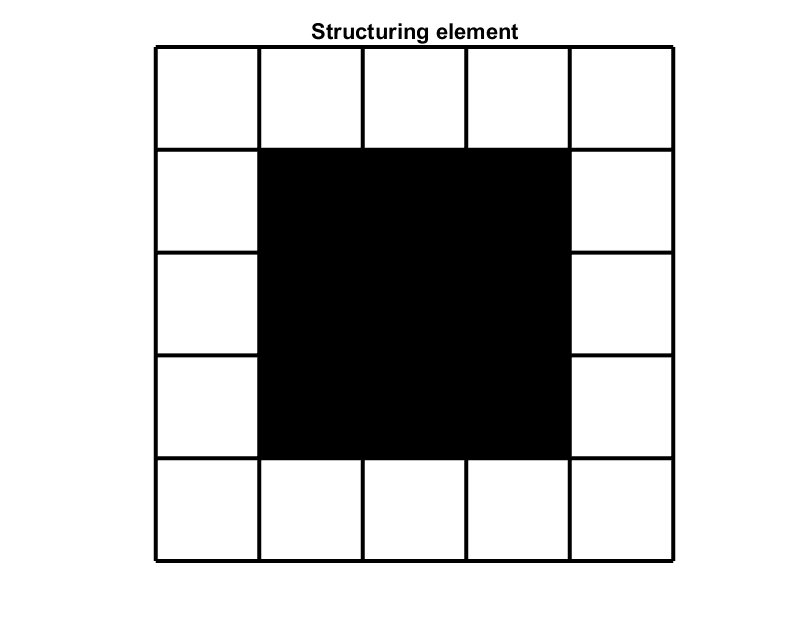
\includegraphics[width=0.6\linewidth]{Morphology/StructuringElement}
		\caption[Structuring Element]{A $3 \times 3$ structuring element.}
		\label{fig:structuringelement}
	\end{figure}
\end{frame}

\begin{frame}
	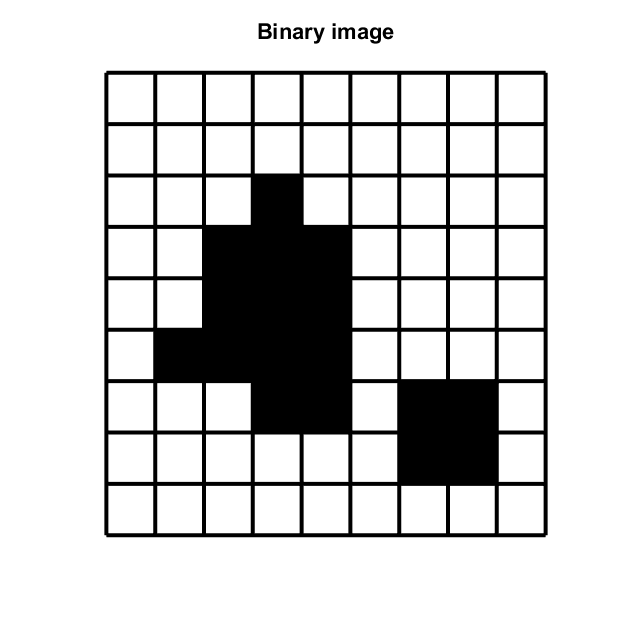
\includegraphics[width=0.3\linewidth]{Morphology/OpeningBefore}
	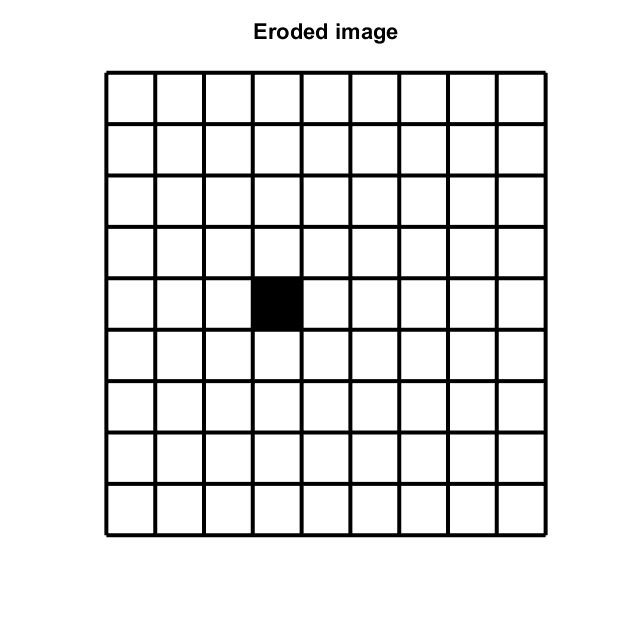
\includegraphics[width=0.3\linewidth]{Morphology/OpeningErode}
	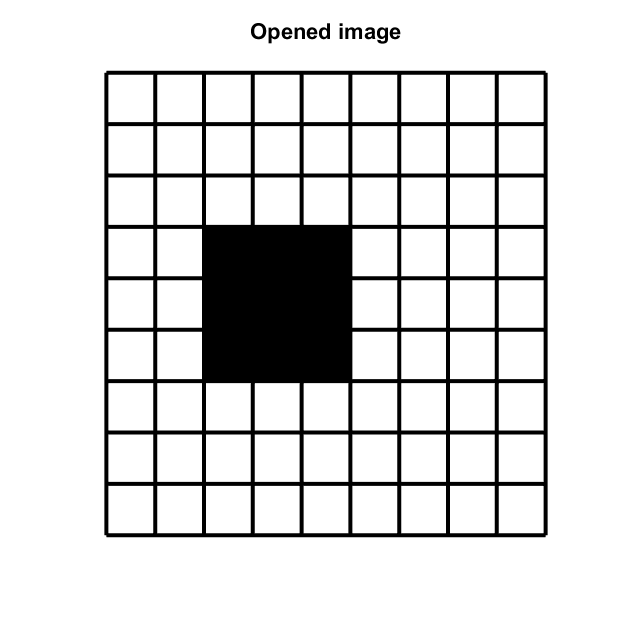
\includegraphics[width=0.3\linewidth]{Morphology/OpeningOpen}
	
	Example of a binary image (black boxes represent 1). The second image is the erosion of the image by a $3 \times 3$ structuring element. The third image is the dilation of the erosion, i.e. the opening of the image.
\end{frame}

\begin{frame}
	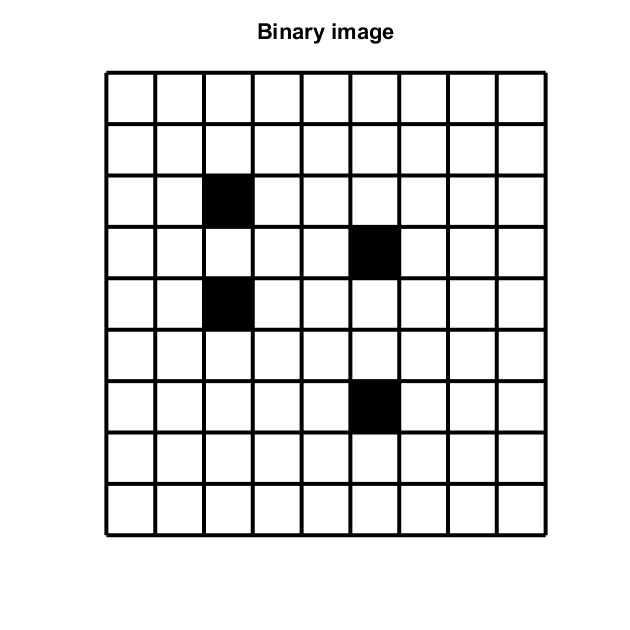
\includegraphics[width=0.3\linewidth]{Morphology/ClosingBefore}
	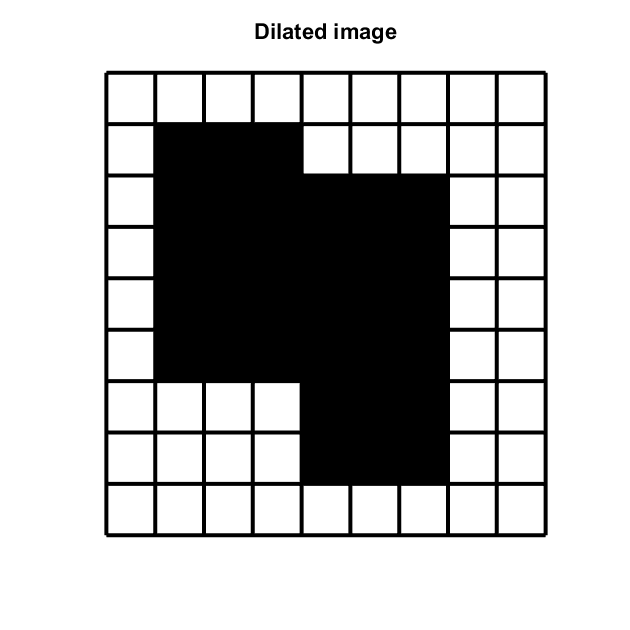
\includegraphics[width=0.3\linewidth]{Morphology/ClosingDilate}
	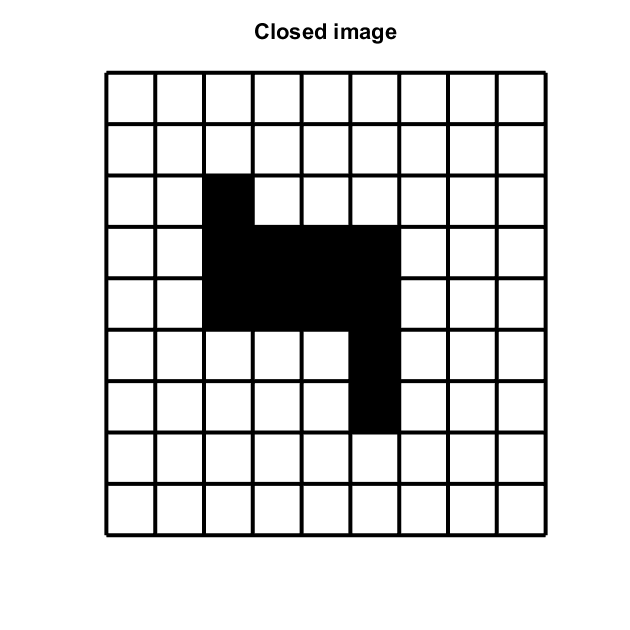
\includegraphics[width=0.3\linewidth]{Morphology/ClosingClosed}
	
	Example of a binary image (black boxes represent 1). The second image is the dilation of the image by a $3 \times 3$ structuring element. The third image is the erosion of the dilation, i.e. the closing of the image.
\end{frame}

\subsection{Hypothesis testing and opening}

\begin{frame}
	\begin{beamercolorbox}[sep=8pt,center,shadow=true,rounded=true]{title}
		Question: What is the effect of opening and closing on statistical significance and power?
	\end{beamercolorbox}
\end{frame}

\begin{frame}
	We will now take a look at the effect of opening on the significance level.
	
	\begin{theorem}
		Let $f$ be an image that contains a rectangular ROI. Assume that we are given a binarized image $f_{bin}$ with
		\begin{equation*}
			\mathbb{P}(f_{bin}(i, j) = 1 \mid H_0(i, j)) \leq \alpha
		\end{equation*}
		where $H_0(i, j)$ denotes the null hypothesis for the pixel $(i, j)$, which is, that it is a background pixel and thus should be set to zero.
		
		Let $k \in \mathbb{N}$ be odd and $B$ be a square structuring element with side length $k$. Then the following inequality holds:
		\begin{equation*}
			\mathbb{P}((f_{bin} \circ B)(i, j) = 1 \mid H_0(i, j)) \leq k^2 \alpha^k
		\end{equation*}
	\end{theorem}
\end{frame}

%\section{Multiple testing procedures}
%
%\begin{frame}
%	Consider the following setup:
%	\begin{table}[h]
%		\tymax .3\textwidth
%		\begin{tabulary}{\textwidth}{|CCCC|}
%			\hline
%			& \textit{Declared non-significant} & \textit{Declared significant} & \textit{Total} \\
%			\hline
%			\textit{True null hypotheses} & $\mathbf{U}$ & $\mathbf{V}$ & $m_0$ \\
%			\textit{Non-true null hypotheses} & $\mathbf{T}$ & $\mathbf{S}$ & $m - m_0$ \\
%			& $m - \mathbf{R}$ & $\mathbf{R}$ & $m$ \\
%			\hline
%		\end{tabulary}
%	\end{table}
%\end{frame}
%
%\begin{frame}
%	\begin{itemize}
%		\item $m$ is the total number hypotheses tested
%		\item $m_0$ is the number of true null hypotheses, an unknown parameter
%		\item $m - m_0$ is the number of true alternative hypotheses
%		\item $V$ is the number of false positives (Type I error) (also called "false discoveries")
%		\item $S$ is the number of true positives
%		\item $T$ is the number of false negatives (Type II error)
%		\item $U$ is the number of true negatives
%		\item $R = V + S$ is the number of rejected null hypotheses (also called "discoveries", either true or false)
%	\end{itemize}
%	In $m$ hypothesis tests of which $m_0$ are true null hypotheses, $R$ is an observable random variable, and $S$, $T$, $U$, and $V$ are unobservable random variables.
%\end{frame}
%
%\begin{frame}
%	We define another random variable $Q = \frac{V}{V + S}$, which is the proportion of the rejected null hypotheses which are erroneously rejected. We set $Q = 0$, if $V + S = 0$. Based on this, we define the false discovery rate to be
%	\begin{equation*}
%		FDR = \mathbb{E}(Q) = \mathbb{E} \left( \frac{V}{V + S} \right)
%	\end{equation*}
%	
%	We also define the family-wise error rate to be
%	\begin{equation*}
%		FWER = \mathbb{P}( V \geq 1 ) = 1 - \mathbb{P}( V = 0 )
%	\end{equation*}
%	that is the probability of making one or more type I errors.
%\end{frame}
%
%\begin{frame}
%	Three of these multiple testing procedures are given in detail in the following. The first one controls the false discovery rate at level $\alpha$, i.e.
%	\begin{equation*}
%		FDR = \mathbb{E}(Q) \leq \alpha
%	\end{equation*}
%	
%	The other two procedures control the family-wise error rate at level $\alpha$, i.e.
%	\begin{equation*}
%		FWER = \mathbb{P}( V \geq 1 ) \leq \alpha
%	\end{equation*}
%\end{frame}
%
%\begin{frame}
%	First, we calculate for every pixel $(m, n) \in G$ the $p$-value
%	\begin{equation*}
%		p(m, n) = \exp \left( - \frac{\tilde{d}(m, n)^2}{4 \sigma^2} \right) \geq \mathbb{P}(T \geq \tilde{d}(m, n) \mid H_0)
%	\end{equation*}
%\end{frame}
%
%\subsection{FDR Thresholding}
%
%\begin{frame}
%	\begin{itemize}
%		\item Sort $p$-values in ascending order: $p_{(1)} \leq p_{(2)} \leq \dots \leq p_{(M \cdot N)}$
%		\item Calculate the maximal index $k$, such that $p_{(k)} \leq \frac{k \cdot \alpha}{M \cdot N}$
%		\item Calculate the threshold $\lambda_{k} = 2 \sigma \sqrt{- \log(p_{(k)})}$
%		\item Reject all hypotheses $H_{(i)}$ with $p_{(i)} \leq p_{(k)}$, i.e. all hypotheses with $$\tilde{d}_{(i)} \geq \tilde{d}_{(k)} = \lambda_{k} = 2 \sigma \sqrt{- \log(p_{(k)})}$$
%	\end{itemize}
%\end{frame}
%
%\subsection{Bonferroni Thresholding}
%
%\begin{frame}
%	\begin{itemize}
%		\item Reject all hypotheses $H_{i}$ with $p_{i} \leq \frac{\alpha}{M \cdot N}$, i.e. all hypotheses with $$\tilde{d}_{i} \geq \lambda_k = 2 \sigma \sqrt{- \log \left( \frac{\alpha}{M \cdot N} \right)}$$
%	\end{itemize}
%\end{frame}
%
%\subsection{Hochberg Thresholding}
%
%\begin{frame}
%	\begin{itemize}
%		\item Sort $p$-values in ascending order: $p_{(1)} \leq p_{(2)} \leq \dots \leq p_{(M \cdot N)}$
%		\item Calculate the maximal index $k$, such that $p_{(k)} \leq \frac{\alpha}{M \cdot N - k + 1}$
%		\item Reject all hypotheses $H_{(i)}$ with $p_{(i)} \leq p_{(k)}$, i.e. all hypotheses with $$\tilde{d}_{(i)} \geq \tilde{d}_{(k)} = \lambda_{k} = 2 \sigma \sqrt{- \log(p_{(k)})}$$
%	\end{itemize}
%\end{frame}
%
%\begin{frame}
%	All these methods are defined for actual $p$-values, i.e.
%	\begin{equation*}
%		p(m, n) = \mathbb{P}(T \geq \tilde{d}(m, n) \mid H_0)
%	\end{equation*}
%	In contrast to that, we have taken upper bounds for the $p$-values. This is not an issue though, since by taking upper bounds we might decrease the number of hypotheses we reject. Thus it will not increase the error rate.
%	
%	The threshold has the following interpretation:
%	\begin{itemize}
%		\item If $\tilde{d}(m, n) \geq \lambda_{k}$, then $(m, n)$ is part of the ROI.
%		\item If $\tilde{d}(m, n) < \lambda_{k}$, then $(m, n)$ is NOT part of the ROI.
%	\end{itemize}
%\end{frame}


\end{document}
